
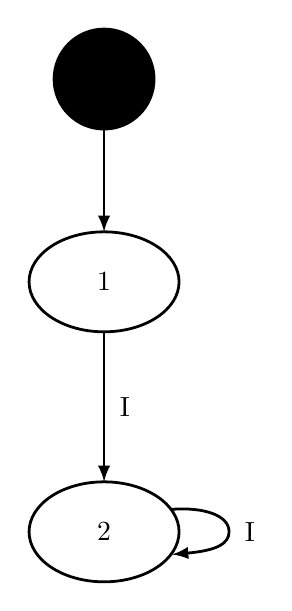
\begin{tikzpicture}[>=latex,line join=bevel,]
  \pgfsetlinewidth{1bp}
%%
\pgfsetcolor{black}
  % Edge: 0 -> 1
  \draw [->] (27bp,162.81bp) .. controls (27bp,154.79bp) and (27bp,145.05bp)  .. (27bp,126.03bp);
  % Edge: 1 -> 2
  \draw [->] (27bp,89.614bp) .. controls (27bp,77.24bp) and (27bp,60.369bp)  .. (27bp,36.05bp);
  \definecolor{strokecol}{rgb}{0.0,0.0,0.0};
  \pgfsetstrokecolor{strokecol}
  \draw (34.5bp,63bp) node {I};
  % Edge: 2 -> 2
  \draw [->] (51.532bp,26.121bp) .. controls (62.508bp,26.895bp) and (72bp,24.188bp)  .. (72bp,18bp) .. controls (72bp,13.843bp) and (67.715bp,11.257bp)  .. (51.532bp,9.8789bp);
  \draw (79.5bp,18bp) node {I};
  % Node: 1
\begin{scope}
  \definecolor{strokecol}{rgb}{0.0,0.0,0.0};
  \pgfsetstrokecolor{strokecol}
  \draw (27bp,108bp) ellipse (27bp and 18bp);
  \draw (27bp,108bp) node {1};
\end{scope}
  % Node: 0
\begin{scope}
  \definecolor{strokecol}{rgb}{0.0,0.0,0.0};
  \pgfsetstrokecolor{strokecol}
  \definecolor{fillcol}{rgb}{0.0,0.0,0.0};
  \pgfsetfillcolor{fillcol}
  \filldraw [opacity=1] (27bp,181bp) ellipse (18bp and 18bp);
\end{scope}
  % Node: 2
\begin{scope}
  \definecolor{strokecol}{rgb}{0.0,0.0,0.0};
  \pgfsetstrokecolor{strokecol}
  \draw (27bp,18bp) ellipse (27bp and 18bp);
  \draw (27bp,18bp) node {2};
\end{scope}
%
\end{tikzpicture}

